\chapter{Implementation}
\chlab{implementation}

A system for fragment-based molecule parameterisation has three distinct tasks: visualising a molecule, finding matching fragments for that molecule, and allowing for interaction with the molecule and its matching fragments. As these tasks can be performed in isolation, it has been decided to implement the molecule parameterisation tool as three separate systems.

The front-end of the system, where users will carry out the parameterisation process, will be called the Online tool for Fragment-based Molecule Parameterisation~(\oframp). This name will also be used to refer to the system as a whole, as it is the hart of the system and is dependent on the other systems. The molecule is also visualised in \oframp, but the for this purpose essential, calculations of atom positions are done in the Online tool for Atom Position Calculations~(\oapoc). Finally, finding matching fragments and sorting them based on relevance is done by the Online tool for Molecule Fragment Finding~(\omfraf).

The complete network diagram for the fragment-based molecule parameterisation system is shown in \figref{network_diagram}. It is clear that \oframp{} is the central system, but that the more computation-intensive tasks are carried out by \oapoc{} and \omfraf{}. The remainder of this chapter will discuss each of the systems in more detail.


\begin{sidewaysfigure}[p]
\begin{center}
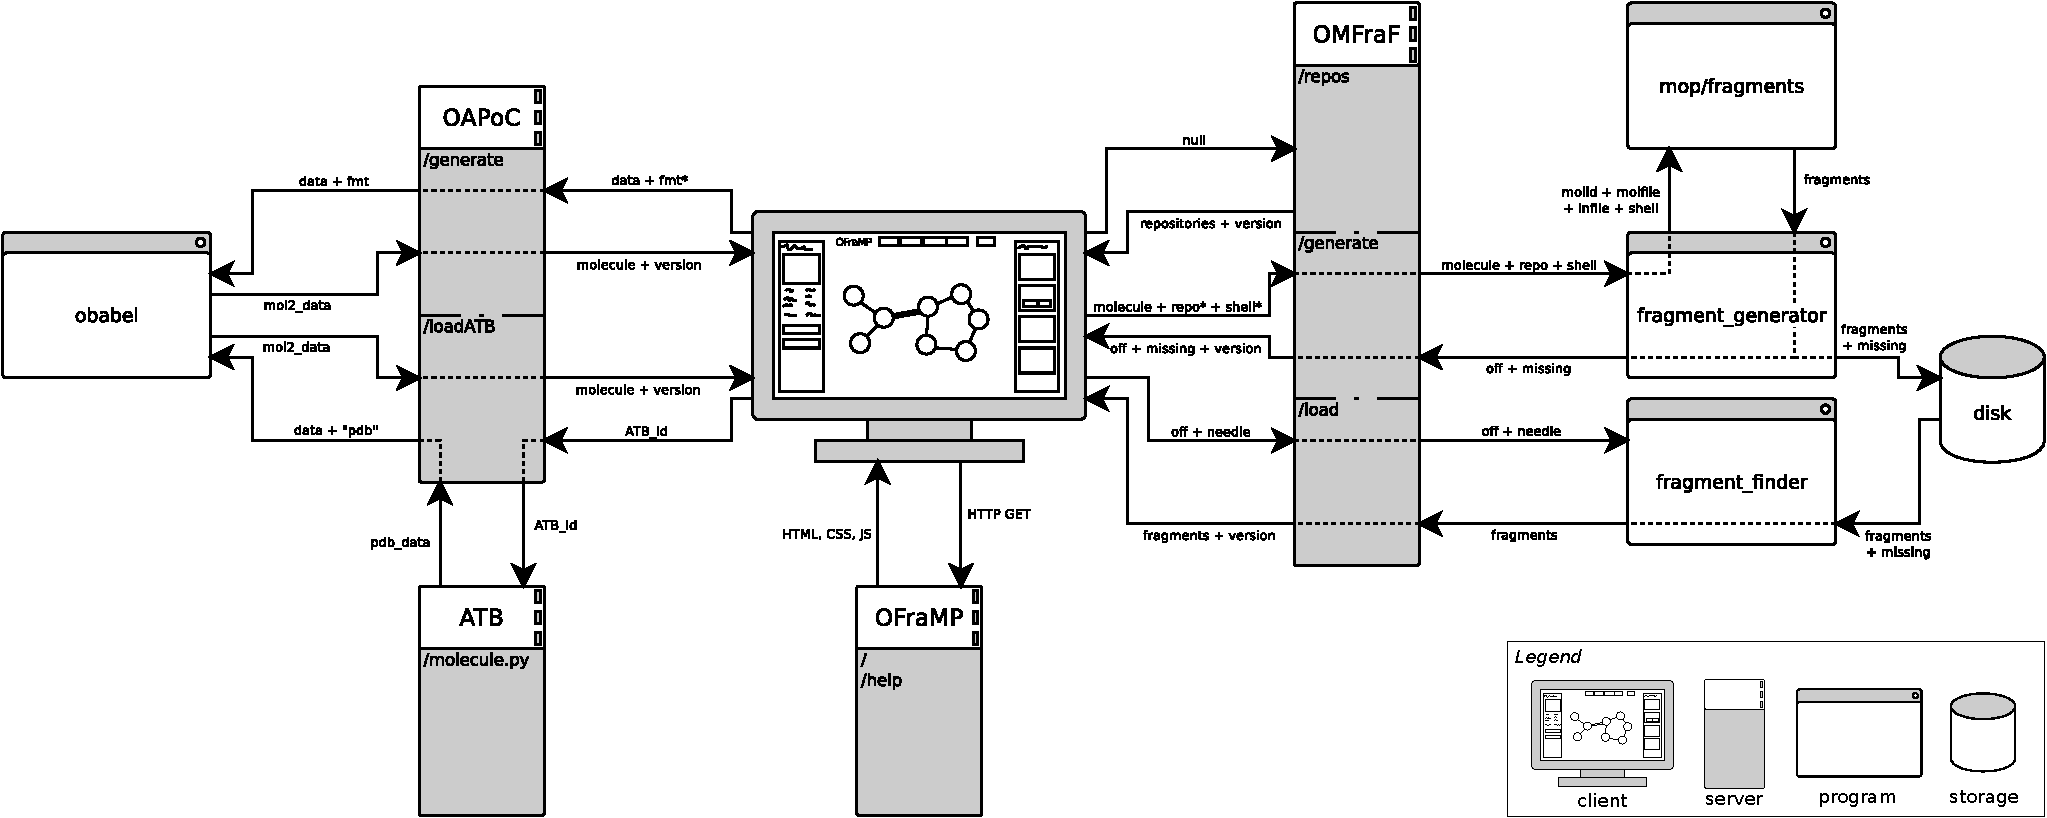
\includegraphics[width=\textwidth]{img/network_diagram.pdf}
\vspace{1em}
\caption{Network diagram of \oframp and its supporting systems.}
\figlab{network_diagram}
\end{center}
\end{sidewaysfigure}


\section[\oframp]{The Online tool for Fragment-based Molecule Parameterisation}
\oframp{} is the central part of the fragment-based molecule parameterisation system. It contains the user interface and connects with \oapoc{} and \omfraf{}. As discussed in \secref{platform}, it has been decided to implement the system as a web application. Following the current trend in web applications, \oframp{} has been implemented using the latest techniques from \verb|HTML5|, \verb|CSS3| and \verb|JavaScript|.

Using the latest web technologies allows for great cross-platform support. It allows the system to run on any desktop and laptop operating system, and creates the possibility of running it on a smartphone or tablet\footnote{This has not been a requirement for the project and has therefore not been tested extensively.}, without requiring any modifications. Still, of course, the limited size of a smartphone screen can be problematic, but it can at least run.

Making use of the latest \verb|HTML5| technologies, however, also comes at a cost. Older browsers generally lack support, and will therefore not be able to run \oframp. Luckily, according to the latest browser statistics from StatCounter~\cite{statcounter2014statcounter}, almost 85\% of internet users uses a browser that has full support for these technologies. Thanks to many compatibility libraries and especially the Internet Explorer \verb|canvas| fallback \verb|excanvas|~\cite{arvidsson2009explorercanvas}, partial support can be provided for browsers used by an additional 11\% of people. In total, this means that 96\% of internet users should be able to run \oframp. A complete list of system requirements can be found in \secref{client_req}.

\subsection{Getting started}

\begin{figure}[b!]
\begin{center}
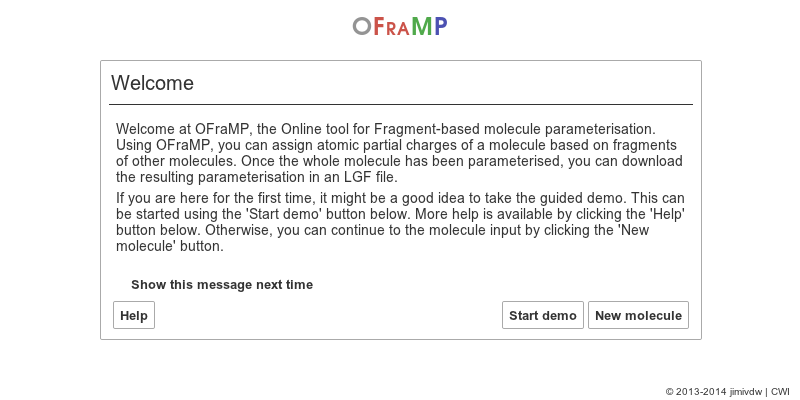
\includegraphics[width=.9\textwidth]{img/impl_welcome.png}
\caption{\oframp{} welcome screen.}
\figlab{impl_welcome}
\end{center}
\end{figure}

Upon loading \oframp{} for the first time, one should see something similar to what is shown in \figref{impl_welcome}. It is explained what the tool is, and what it should be used for. Additionally, instructions are provided for first-time users and pointers are provided to the help pages. From this point, users can either start a short demonstration guide~(see \secref{impl_demo}) or submit a new molecule into the system~(see \secref{impl_inserting}).

\Figref{impl_welcome} also shows the basic design of the system. It has been decided to go for a minimal look with a simple, purely textual logo. Besides the pastel colours of the logo, all text uses a dark shade of grey. Boxes and buttons all have a white background and a light grey, slightly rounded border.

Overly designed shiny elements are known to distract the user from his tasks~\cite{norman1990interfaces}~(see also \secref{design}). In some cases this may be beneficial, but for the purpose of finding a good molecule parameterisation this is undesirable. Therefore, this minimal design tries to make sure the user stays focused on the task that he needs to perform, rather than on using the tool. Furthermore, the tool still looks good and decent, which should prevent the users from distrusting it due to poor design~\cite{norman2002emotion}~(see also \secref{design}).

\subsubsection{Submitting a molecule}
\seclab{impl_inserting}

\begin{figure}[t!]
\begin{center}
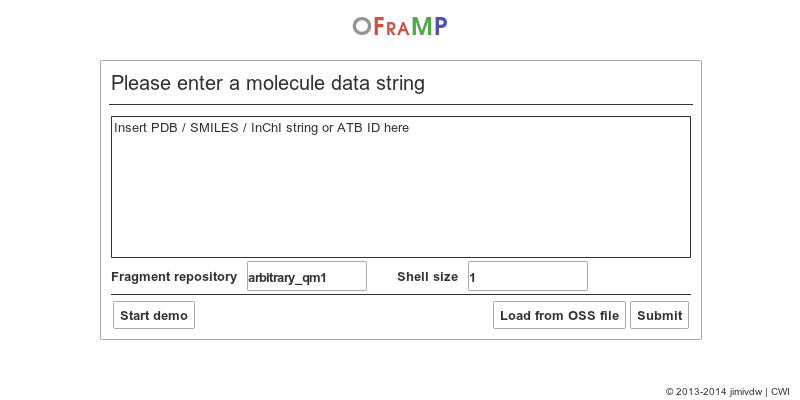
\includegraphics[width=.9\textwidth]{img/impl_inserting.png}
\caption{Insertion window for molecule data strings.}
\figlab{impl_inserting}
\end{center}
\end{figure}

In \figref{impl_inserting}, the insertion window for molecules is shown. This is where users should submit the molecules in a machine readable format, the so called molecule data string~(MDS). As discussed before, the system supports the \verb|PDB|, \verb|SMILES|, and \verb|InChI| formats, and the use of \verb|ATB ID|s~(see \secref{id_common}). When the MDS has been entered, the user can click the `Submit' button, after which the molecule will be displayed~(see \secref{impl_visualisation}).

Additionally, the user can adjust the fragment repository and shell size that are to be used for finding matching fragments of other molecules. The available repositories are retrieved from \omfraf~(see \secref{impl_omfraf}). This will be explained in more detail in \secref{impl_generating}. Furthermore, the demonstration mode~(see \secref{impl_demo}) can be started from this window as well, in case the user accidentally clicked the wrong button in the previous step. Finally, the user can load a so called \oframp{} State Storage~(OSS) file. These files can be created at any point in the parameterisation process and will store all progress up until that point. They can be loaded again at a later stage to continue the parameterisation process from that point.


\subsection{Visualisation}
\seclab{impl_visualisation}
Once a molecule data string has been entered into the system, the positions of its atoms and the connections between them are retrieved from \oapoc~(see \secref{impl_oapoc}). This data is then transformed to a \verb|JavaScript| \verb|Molecule| instance, as can be seen in \figref{oframp_class}. \verb|Molecule| instances can be visualised using a \verb|MoleculeViewer|, which will draw the molecule onto an \verb|HTML| \verb|canvas|.

\begin{figure}[t!]
\begin{center}
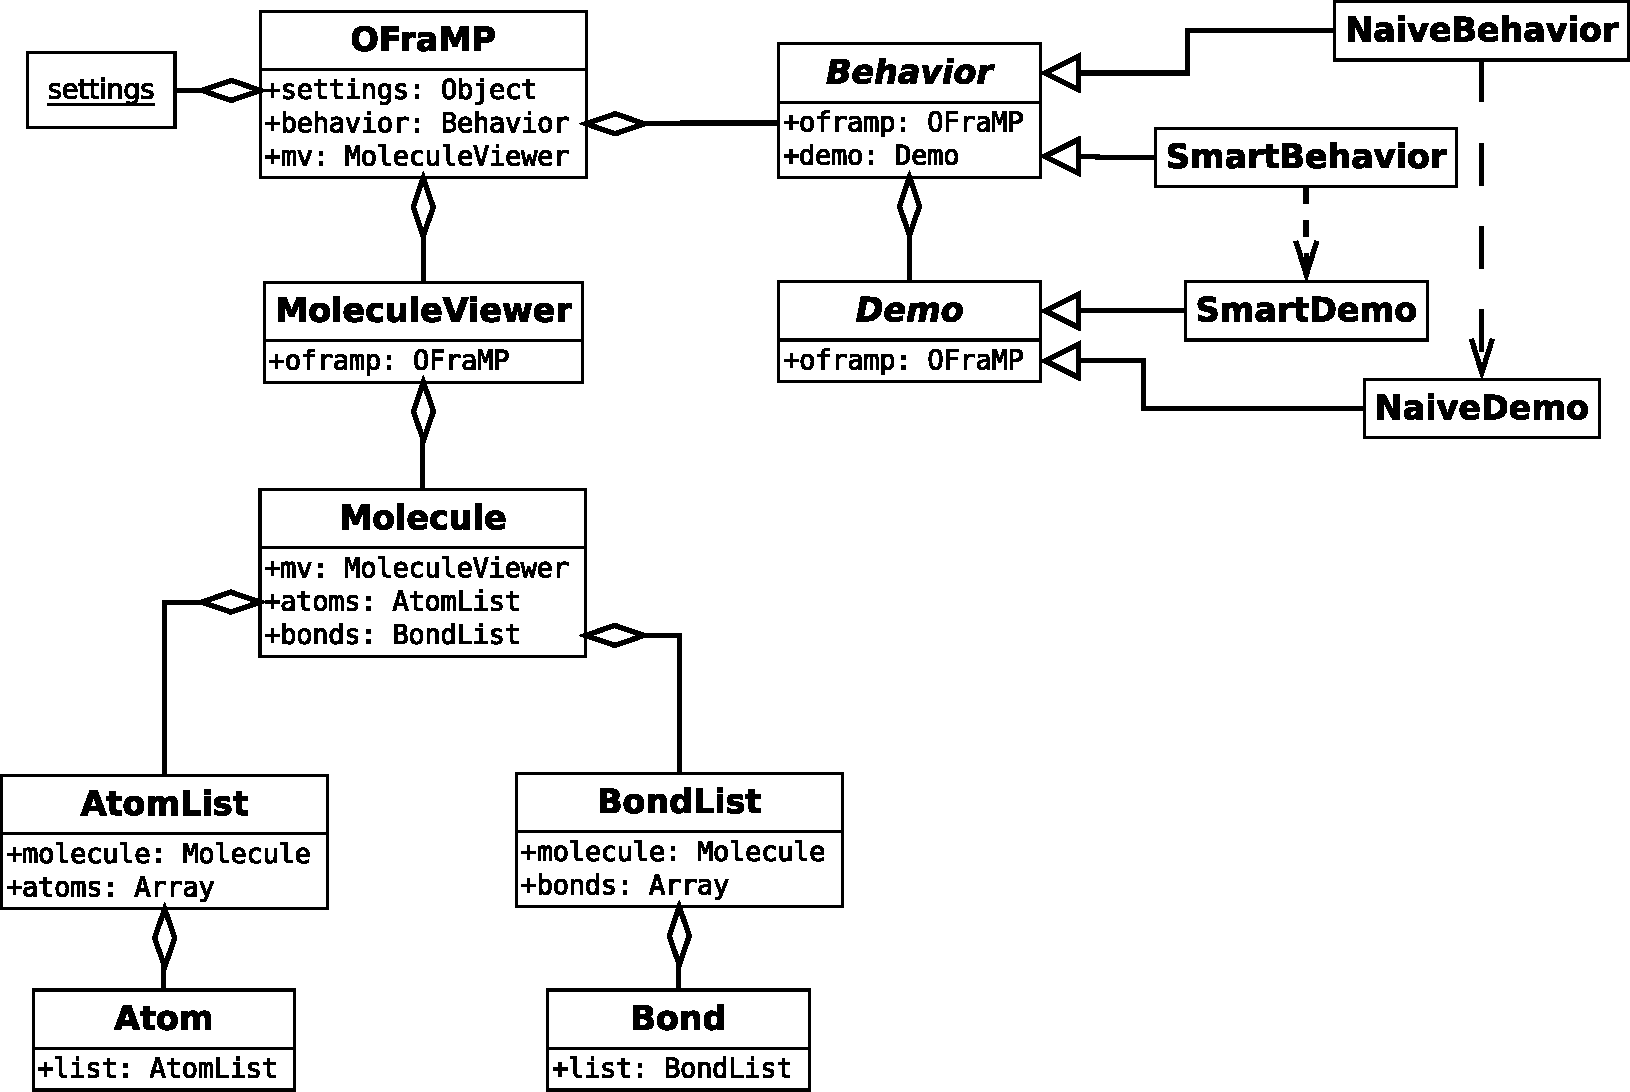
\includegraphics[width=\textwidth]{img/oframp_class.pdf}
\caption{Simplified class diagram of \oframp.}
\figlab{oframp_class}
\end{center}
\end{figure}

Upon entering the \verb|SMILES| MDS \verb|NCC(=O)CCO| into \oframp, one should see something resembling what is shown in \figref{impl_visualising}. Similar to the molecule visualisation of the ATB~(see \figref{partial_charges} on \figpageref{partial_charges}), atoms are displayed as circles containing the atom type and with connecting lines that denote bonds. However, there are also a number of differences. First of all, charge group information is missing here, as these cannot be found before the atomic charges are available. Second, atom IDs (both on molecule and type scale) are left out. These are not considered to add any helpful information, and can therefore only be confusing. Third, obviously, the atom charges are missing, as they have not yet been assigned. As soon as a matching fragment is selected, they will also be added to the visualisation~(see \secref{impl_parameterisation}). Fourth, as can be seen at the bottom-most \verb|O| atom, double bonds are visualised properly as a double line. The same is true for triple bonds that show as a triple line, and aromatic bonds that are indicated with a dotted line on the inside of the aromatic cycle they are a part of~(see also \secref{ormaybeanimage}).

\begin{figure}[b!]
\begin{center}
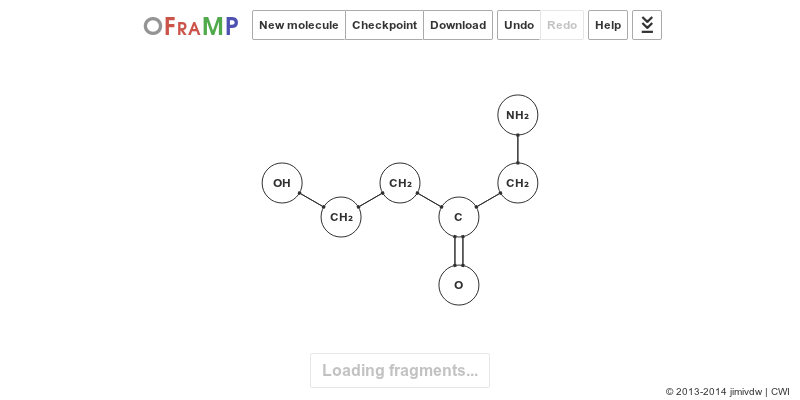
\includegraphics[width=.9\textwidth]{img/impl_visualising.png}
\caption{\oframp{} visualisation of \texttt{NCC(=O)CCO}.}
\figlab{impl_visualising}
\end{center}
\end{figure}

Finally, what is probably the most notable difference, is the fact that the \verb|H| atoms are grouped with their base atoms\footnote{This, along with many other settings, can be altered. See \secref{impl_settings} for more information.}. This means that they do not need to be drawn separately, leaving more space around the other atoms, thereby enhancing the overview of the complete molecule. Furthermore, in chemistry, it is quite common to have this combination and, in many calculations, these groups can be treated as a single atom. As this does not hold for other atom types, those will not be grouped in the \oframp{} visualisation, to ensure chemical correctness.

\subsubsection{Interaction}
At this point, the molecule can already be interacted with. It can be moved around by holding down the \emph{left} mouse button and dragging the mouse. This is mostly useful for larger molecules that may not completely fit on smaller screens. To provide further support for large molecules, the user has the opportunity to zoom in on certain sections of the molecule, or zoom out to make more atoms fit on the screen. Zooming can be done using the mouse wheel, or the zoom buttons located in the advanced controls settings, which can be opened using the button with the down pointing arrow~(see \figref{impl_visualising}).


\subsubsection{Deoverlapping}
As discussed in \secref{ms_visualisation} and~\cite{clark2006structure}, overlap in atoms and bonds still occurs in modern molecule visualisation software. In this case, where the atoms have a relatively large radius to make room for displaying the charge, chances are even higher. To temper the effects of this, a simple deoverlap algorithm has been implemented. \Figref{impl_deoverlap} shows the three different types of deoverlapping that \oframp{} can do. Here, the light blue line indicates a vector that is used to determine if there is any overlap, the red line indicates the overlapping part, and the green arrow~(of equal length to the red line) shows where the atom centre should be moved to in order to resolve the overlap.

\begin{figure}[b!]
\begin{center}
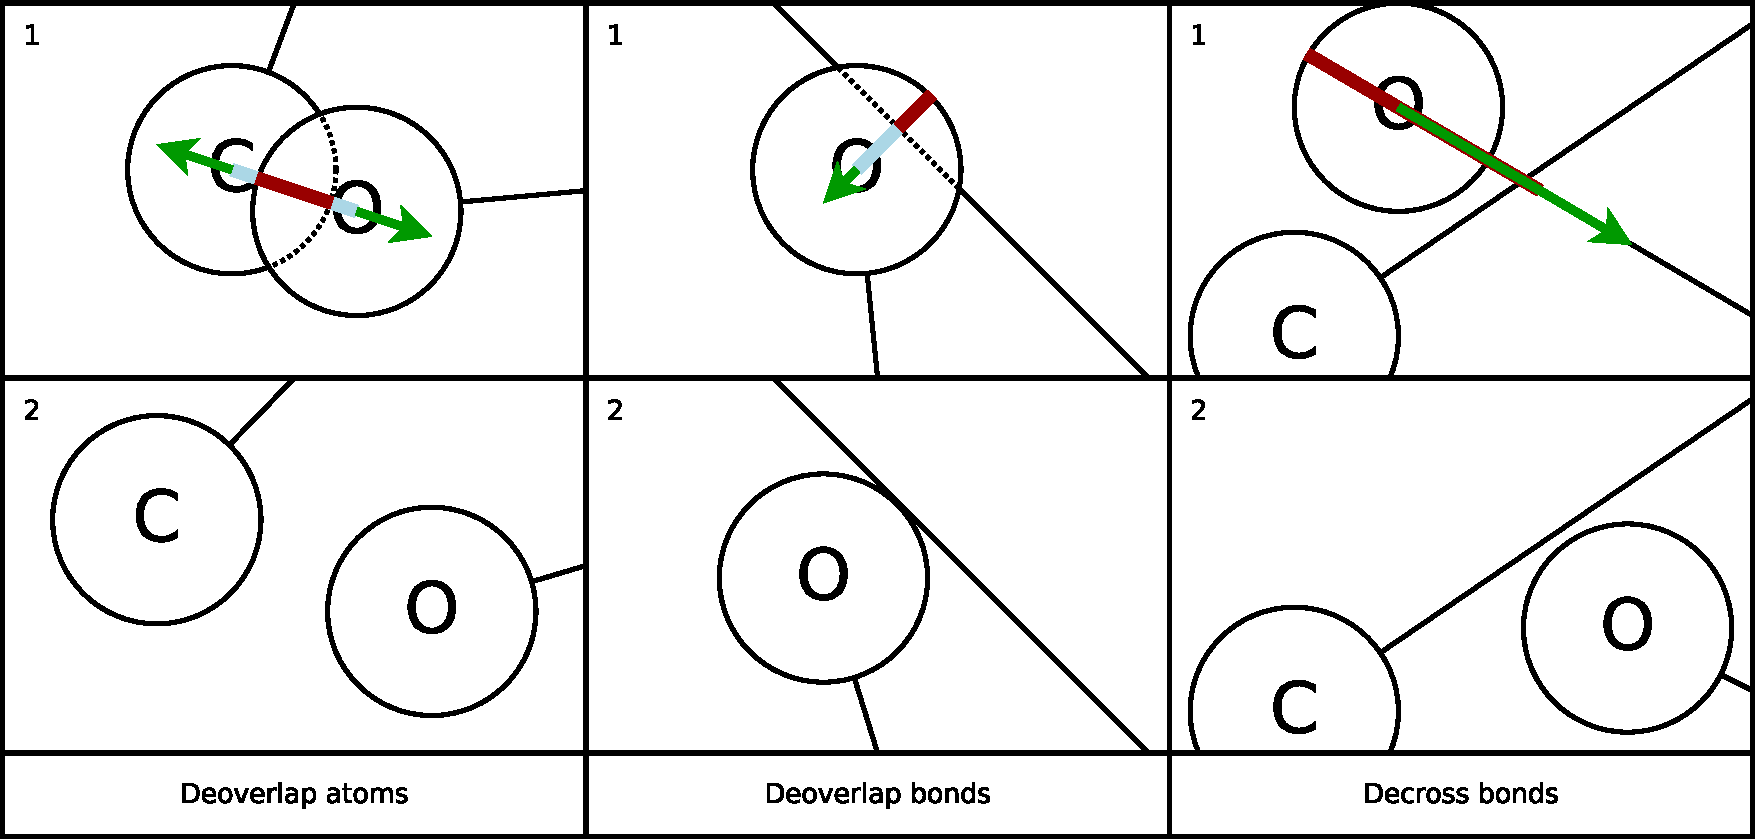
\includegraphics[width=\textwidth]{img/deoverlap.pdf}
\caption{Concepts of deoverlap.}
\figlab{impl_deoverlap}
\end{center}
\end{figure}

By default, for performance reasons, only the deoverlapping of atoms is enabled. This is the easiest to detect and solve, but also the most important one. Atoms that overlap almost entirely might not be spotted by the user, and atom types and charges may become hidden due to another atom lying on top of them. As can be seen in \figref{impl_deoverlap}, this type of deoverlap works by calculating the distance between the two atom centres and subtracting the atom radius from that twice~(once for each atom). If this distance is smaller than $0$, both atom centres will be moved along the line that connects the two for a distance that is equal to the overlap distance. This ensures that the atoms will no longer overlap, and even creates some room between them.

In order to solve atoms overlapping bonds, the perpendicular distance from the atom centre to the bond needs to be calculated. When this distance is smaller than the atom radius, the atom needs to be moved along the perpendicular for a distance that is equal to the overlap distance. This will put the atom right next to the bond.

The third and final type of deoverlapping, the so-called decrossing of bonds, is also the hardest one. First, it needs to be determined if the two bonds intersect each other. When that is the case, the intersection point needs to be found. The overlap distance here is equal to the distance from the atom centre to the intersection point, plus the radius of the atom. The atom then needs to be moved along its bond for a distance that is equal to the overlap distance, in order to solve the crossing bonds.

Unfortunately, solving one occurrence of overlap could result in overlap occurring in a different place, as moving an atom could potentially move it on top of another. Therefore, the deoverlap process will need to repeat itself to solve all overlap in the molecule. However, it is possible that the solution of one overlap occurrence is the exact opposite of another, which means that, after two iterations, the situation will be exactly the same as it was initially. In order to prevent the deoverlap process from going into an endless loop because of this, a time limit~(set to half a second by default) has been built in, after which the deoverlapping will stop.

\subsection{Parameterisation}
\seclab{impl_parameterisation}

\nlipsum

\subsubsection{Manual `naive' version}
\nlipsum

\subsubsection{Semi-automatic `smart' version}
\nlipsum


\subsection{Fine-tuning charges}
\nlipsum


\subsection{Wrapping up}
We use LGF files~\cite{dezso2011lemon}\ldots

\nlipsum


\subsection{Other features}
\nlipsum

\subsubsection{Demo mode}
\seclab{impl_demo}
\nlipsum

\subsubsection{Help}
\nlipsum

\subsubsection{Modifying visualisation parameters}
\seclab{impl_settings}
\nlipsum


\section[\oapoc]{The Online tool for Atom Position Calculations}
\seclab{impl_oapoc}
\nlipsum

\subsection{From ATB}
\nlipsum

\subsection{obabel}
\nlipsum


\section[\omfraf]{The Online tool for Molecule Fragment Finding}
\seclab{impl_omfraf}
\nlipsum

\subsection{Getting the repositories}
 by sending an empty \verb|JSON| object to its \verb|/repos| URL~(see \figref{network_diagram})
\nlipsum

\subsection{Generating fragments}
\seclab{impl_generating}
\nlipsum

\subsubsection{mop/fragments}
\nlipsum

\subsection{Finding fragments}
\nlipsum
